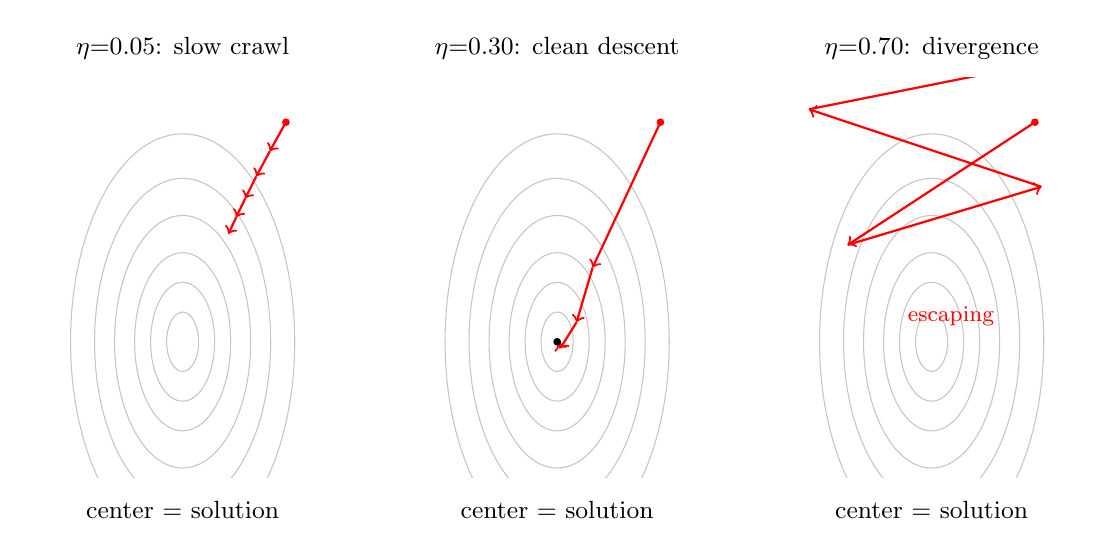
\begin{tikzpicture}[scale=0.82]
% small multiples: GD trajectories on same quadratic contours
% contours of f on [-0.5,2.5]x[-0.5,2.5] around (-0.5,2.5)
\foreach \xo/\et/\cap in {0/0.05/{$\eta{=}0.05$: slow crawl},5.8/0.30/{$\eta{=}0.30$: clean descent},11.6/0.70/{$\eta{=}0.70$: divergence}}{
\begin{scope}[xshift=\xo cm]
\clip (-2.4,-2.1) rectangle (2.4,4.1);
\foreach \r in {0.4,0.8,1.2,1.7,2.2,2.8}
  \draw[gray!45] (0,0) ellipse [x radius=\r*0.62, y radius=\r*1.15];
\end{scope}
\node at (\xo+0,4.55) {\small \cap};
\node at (\xo+0,-2.6) {\small center = solution};
}
% eta=0.05: slow monotone crawl (real iterate pattern)
\begin{scope}
\clip (-2.4,-2.1) rectangle (2.4,4.1);
\draw[thick,red,->] (1.6,3.4) -- (1.35,2.95);
\draw[thick,red,->] (1.35,2.95) -- (1.14,2.56);
\draw[thick,red,->] (1.14,2.56) -- (0.97,2.22);
\draw[thick,red,->] (0.97,2.22) -- (0.83,1.93);
\draw[thick,red,->] (0.83,1.93) -- (0.71,1.67);
\fill[red] (1.6,3.4) circle (1.7pt);
\end{scope}
% eta=0.30: zig-zag but converging
\begin{scope}[xshift=5.8cm]
\clip (-2.4,-2.1) rectangle (2.4,4.1);
\draw[thick,red,->] (1.6,3.4) -- (0.55,1.15);
\draw[thick,red,->] (0.55,1.15) -- (0.30,0.30);
\draw[thick,red,->] (0.30,0.30) -- (0.05,-0.10);
\draw[thick,red,->] (0.05,-0.10) -- (0.02,-0.02);
\fill[red] (1.6,3.4) circle (1.7pt);
\fill[black] (0,0) circle (1.7pt);
\end{scope}
% eta=0.70: bouncing out
\begin{scope}[xshift=11.6cm]
\clip (-2.4,-2.1) rectangle (2.4,4.1);
\draw[thick,red,->] (1.6,3.4) -- (-1.3,1.5);
\draw[thick,red,->] (-1.3,1.5) -- (1.7,2.4);
\draw[thick,red,->] (1.7,2.4) -- (-1.9,3.6);
\draw[thick,red,->] (-1.9,3.6) -- (2.1,4.4);
\fill[red] (1.6,3.4) circle (1.7pt);
\node[red] at (0.3,0.4) {\footnotesize escaping};
\end{scope}
\end{tikzpicture}
